\documentclass[a4paper, 12pt]{article}

%%% Работа с русским языком
\usepackage{cmap}					% поиск в PDF
\usepackage{mathtext} 				% русские буквы в формулах
\usepackage[T2A]{fontenc}			% кодировка
\usepackage[utf8]{inputenc}			% кодировка исходного текста
\usepackage[russian]{babel}	% локализация и переносы

%%% Дополнительная работа с математикой
\usepackage{amsmath,amsfonts,amssymb,amsthm,mathtools} % AMS
\usepackage{icomma} % "Умная" запятая: $0,2$ --- число, $0, 2$ --- перечисление

%% Номера формул
%\mathtoolsset{showonlyrefs=true} % Показывать номера только у тех формул, на которые есть \eqref{} в тексте.

%% Шрифты
\usepackage{euscript}	 % Шрифт Евклид
\usepackage{mathrsfs} % Красивый матшрифт

%% Поля
\usepackage[left=2cm,right=2cm,top=2cm,bottom=2cm,bindingoffset=0cm]{geometry}

%% Русские списки
\usepackage{enumitem}
\makeatletter
\AddEnumerateCounter{\asbuk}{\russian@alph}{щ}
\makeatother

%%% Работа с картинками
\usepackage{graphicx}  % Для вставки рисунков
\graphicspath{{images/}{images2/}}  % папки с картинками
\setlength\fboxsep{3pt} % Отступ рамки \fbox{} от рисунка
\setlength\fboxrule{1pt} % Толщина линий рамки \fbox{}
\usepackage{wrapfig} % Обтекание рисунков и таблиц текстом

%%% Работа с таблицами
\usepackage{array,tabularx,tabulary,booktabs} % Дополнительная работа с таблицами
\usepackage{longtable}  % Длинные таблицы
\usepackage{multirow} % Слияние строк в таблице
\usepackage[table,xcdraw]{xcolor} % Цветные таблицы

%% Красная строка
\setlength{\parindent}{2em}

%% Интервалы
\linespread{1}
\usepackage{multirow}

%% TikZ
\usepackage{tikz}
\usetikzlibrary{graphs,graphs.standard}

%% Верхний колонтитул
\usepackage{fancyhdr}
\pagestyle{fancy}

%% Перенос знаков в формулах (по Львовскому)
\newcommand*{\hm}[1]{#1\nobreak\discretionary{}
	{\hbox{$\mathsurround=0pt #1$}}{}}

%% Мои дополнения
\usepackage{float} %Добавляет возможность работы с командой [H] которая улучшает расположение на странице
\usepackage{gensymb} %Красивые градусы
\usepackage{graphicx}               % Импорт изображений
\usepackage{caption} % Пакет для подписей к рисункам, в частности, для работы caption*


\begin{document}

\newcommand{\HRule}{\rule{\linewidth}{0.7mm}} % Defines a new command for the horizontal lines, change thickness here
	
	\begin{center}
		\large\textbf{Московский Физико-Технический Институт}\\
		\large\textbf{(государственный университет)}
	
		\vfill
		
		\Large Лабораторная работа по радиотехническим сигналам и цепям № 20\\[0.5cm] % Minor heading such as course title
		
		%----------------------------------------------------------------------------------------
		%	TITLE SECTION
		%----------------------------------------------------------------------------------------
		
		\HRule
		\\[0.4cm]
		{ \huge \bfseries Связанные колебательные контуры}
		\\[0.4cm] % Title of your document
		\HRule
		\\[0.5cm]
		
		\ \\
	\textbf{\large Автор:} \\	
	\large Баранников Андрей Б01-001\\
	\textbf{\large Преподаватель:} \\
	\large Григорьев Иван Александрович\\
		\vfill
		\hspace*{-0.8 cm}
\includegraphics[width=100 pt]{frkt_logo}\\
		\large Долгопрудный, 2021
	\end{center}

\newpage
\setcounter{page}{2}
\fancyfoot[c]{\thepage}
\fancyhead[L] {Работа № 20}
\fancyhead[R]{}

\newpage

\begin{figure}[H]
	\centering
	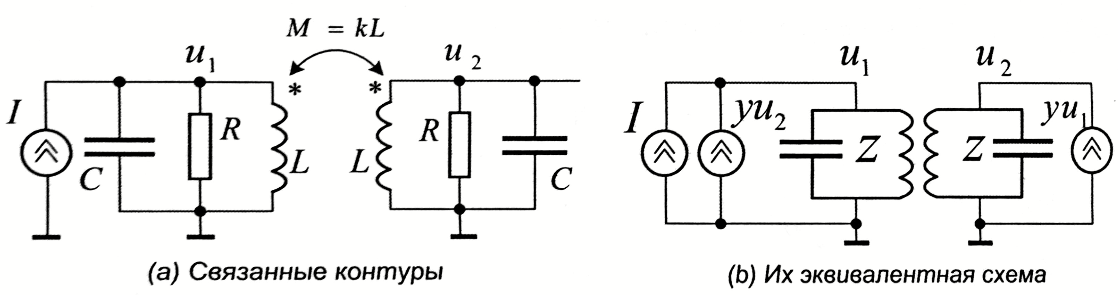
\includegraphics[width =  0.9\linewidth]{image_1}
	\caption{Связанные контуры.}
\end{figure}

\section*{Задание №1. Система с индуктивной связью.}

\textbf{3.} Изучим поведение резонансных кривых и фазовых характеристик при $F = [0.2, 1|0.2]$ и $F = [1.5|1]$. Измерим границы диапазонов изменения фаз на первом и втором контурах: 
\begin{itemize}
\item На первом контуре $ \varphi $:   от $-84.7^{\circ}$ до $83.5^{\circ}$ \\
		На втором контуре $ \varphi $: от $-258.2^{\circ}$ до $77.1^{\circ}$ 
\item Разность фаз между напряжениями на контурах на частоте $\Delta \varphi (f_0)$: $89.8^{\circ}$.

\item Измерив уровни $u_1(f_0)$, $u_2(f_0)$ при $F = 0.5, 1, 2$, проверим формулы:
\begin{equation}
	\label{f1}
	u_1(f_0) = \frac{1}{1+F^2} \quad \quad u_2(f_0)= \frac{F}{1+F^2}
\end{equation}

\begin{table}[H]
	\centering
	\begin{tabular}{|c|c|c|c|} \hline
		$F$                         & $0.5$ & $1$ & $2$ \\ \hline
		$u_1(f_0)_{эксп}$          & 0.8 & 0.5   & 0.2 \\ \hline
		$u_1(f_0)_{теор}$ & 0.8 & 0.5   & 0.2 \\ \hline
		$u_2(f_0)_{эксп}$          & 0.4 & 0.5   & 0.2 \\ \hline
		$u_2(f_0)_{теор}$ & 0.4 & 0.5   & 0.2 \\ \hline
	\end{tabular}
	\caption{Проверка формулы уровней $ u_1(f_0) $ и $ u_2(f_0) $}
\end{table}

По результатам измерений можно сделать вывод, что формула \textit{выполняется}.

\end{itemize}
\textbf{4.} Измерим значения $F$, при которых возникает: 
\begin{itemize}
\item Провал на первом контуре: $F = 0.6$
\item Провал на втором контуре: $F = 1.1$ 
\item Подъём на фазовой характеристике первого контура: $F = 1$.
\item Измерим частоты пересечения нуля фазовой характеристикой $u_1$ при $F = 5$ ($\nu \hm{=} 975.9k,~1.001M,~1.025M$) и при $F = 10$ ( $\nu = 953.5k,~1.005M,~1.054M$). 
\item По приближенной ($ f_0 \pm FF_0 $) и уточнённой ($ f_0\sqrt{1 \pm \frac{F}{Q}} $) формулам: \\
		F = 5: $ (1000 \pm 25) \ k \ \ | \ \ (1000\sqrt{1 \pm 0,05}) k$   \\  
		F = 10: $ (1000 \pm 50) \ k \ \ | \ \ (1000\sqrt{1 \pm 0,1}) k$

\end{itemize}

\newpage
\textbf{5.} 
\begin{itemize}
\item При критической связи измерим ширину полосы по уровню -3dB эталонного контура ($\Delta f = 10k$) и ширину полосы по уровню -9dB резонансной кривой на втором контуре ($\Delta f = 14.3k$). 
\item Убедимся, что их отношение составляет $\sqrt{2}$:\\
 $$ 10 \ k \cdot \sqrt{2} = 14.14 \ k \approx 14.3 k $$

\item Измерим уровни затухания критической кривой при сдвигах по частоте на декаду $F_0$, то есть на $\pm 10F_0 = \pm 50k$:
\[
\textit{Затухание}  -34\frac{dB}{\text{дек}_{F_0}}. 
\]
\item Варьируя сопротивление потерь эталонного контура $R = [60k,~80k|5k]$, выясним, при какой добротности его полоса сравнивается с полосой двухконтурной системы:
 $$
 Q = 70 \ \ R \hm{=} 70k \ \ \Delta f = 14.1k
 $$ 
 \item Измерим затухание, вносимое эталонным контуром с этой добротностью при расстройках на декаду $F_0$: 
 \[
 \textit{Затухание}  -17,1 \frac{dB}{\text{дек}_{F_0}}. 
 \]
 \item В итоге выигрыш духконтурной системы $\simeq~\text{2 раза}$ 

\end{itemize}

\textbf{6.}
\begin{itemize}
 \item Изучим поведение резонансных кривых при $F \hm{=} [0.5,~1|0.1]$. 
 \item Найдём значение $F \hm{=} [0.65,~0.75|0.05]$, при котором полоса двухконтурной системы по критическому уровню -9dB сравнивается с полосой $10k$ эталонного контура: 
 \[
  F = 0.75
 \]

 \item При этом значении $F$ оценим выигрыш по затуханию при расстройке на декаду $F_0$ двухконтурной системы по сравнению с эталоном:
 \[
  \textit{Эталон}:  -19.75\frac{dB}{\text{дек}_{F_0}} \quad \quad \textit{Двухконтурная \ система}: -36.45\frac{dB}{\text{дек}_{F_0}} 
 \]
Соответственно, выигрыш $ \approx $ 2 раза.
\end{itemize}

\textbf{7.} 
\begin{itemize}
	\item Изучим поведение резонансных кривых при $F {=} [1,5|1]$.
	\item Измерим значение $F$ из диапазона $F = [2.2,~2.6|0.1]$, при котором провал на втором контуре касается сверху критического уровня -9dB:
	$$
	F = 2.4
	$$ 
	\item При этом значении $F$ измерим ширину полосы $\Delta \omega$ двухконтурной системы по уровню -9dB и уровни затухания при расстройках на декаду $F_0$: 
	
	\[
		\Delta \omega \approx 30 \ k 
	\]
	\[
		 \textit{Затухание эталона:} -21\frac{dB}{\text{дек}_{F_0}} \quad \quad \textit{Затухание двухконтурной системы:} -26\frac{dB}{\text{дек}_{F_0}}
	\]
	\item Варьированием сопротивления эталонного контура $R$ добьёмся совпадения его полосы с полосой двухконтурной системы и измерим уровни затухания, вносимого контуром:
	$$
	-15\frac{dB}{\text{дек}}
	$$
	Выигрыш по затуханию двухконтурной системы с неравномерностью -3dB в полосе пропускания $ \approx $ 2 раза

\end{itemize}

\textbf{10.}  
\begin{itemize}
	\item В режиме \textit{Transient} проанализируем переходные характеристики до напряжений на первом и втором контурах при F = 1.
	\item Установим F = 0.1 и измерим постоянную времени $ \tau $ экспоненциального спада огибающей напряжения $ u_1 ~ e^{-t/\tau} $ до уровня $ \frac{1}{e} = 0.37 $:
	\[
		\tau_{эксп} \approx 31.5 \ мкс \quad \quad \tau_{теор} \approx 32.0 \ мкс \quad \quad \tau_{эксп} \approx \tau_{теор}
	\]
	
	\begin{table}[!h]
		\centering
		\begin{tabular}{|c|c|}
			\hline
			F & $ \nu $, кГц \\ \hline
			1 & 4,54   \\ \hline
			2 & 9,09   \\ \hline
			4 & 17,86  \\ \hline
			8 & 37,04  \\ \hline
		\end{tabular}
	\end{table}

\end{itemize}
\textbf{11.} Установив диапазон моделирования $[2Meg, 600k]$, исследуем частотные и фазовые характеристики при сильной связи. Измерим частоты $f_{\pm}$ пиков при $F = 50$: 
$$
f_{+} = 1.414M \quad \quad  f_{-} = 818.274k
$$

\newpage

\section*{Задание №2. Система с ёмкостной связью.}
\textbf{1.} Измерим диапазоны изменения фазовых характеристик на первом и втором контурах:

на 1 контуре -- от $90^{\circ}$ до $-90^{\circ}$

на 2 контуре -- от $-90^{\circ}$ до $-450^{\circ}$.

Измерим значения $F$, при которых возникает: 
\begin{itemize}
	\item Провал на первом контуре: $F = 0.5$
	\item Провал на втором контуре: $F = 1$ 
	\item Подъём на фазовой характеристике первого контура: $F = 1$.

Снимем зависимость частоты провала на втором контуре от $F = [2, 4|1]$:

\begin{table}[H]
	\centering
	\begin{tabular}{|c|c|c|c|} \hline
		$F$               & $2$    & $3$    & $4$    \\ \hline
		$f_{\text{пров}},~\text{Гц}$ & $990k$ & $985k$ & $980k$ \\ \hline
	\end{tabular}
\end{table}

\end{itemize}

\textbf{2.} Измерим уровни затухания при расстройках на $\pm 50k$:
\[
1 \ контур: -17 \ \frac{dB}{\text{дек}} \quad \quad 2 \ контур: -35 \ \frac{dB}{\text{дек}}.
\]


Перейдём на частотный диапазон $[10Meg,100k]$ и измерим уровни затухания при расстройках на декаду $f_0$:
\[
1 \ контур: -56 \ \frac{dB}{\text{дек}} \quad \quad  2 \ контур: -94 \ \frac{dB}{\text{дек}}(\text{вблизи 100k}), -133 \ \frac{dB}{\text{дек}}(\text{вблизи 10Meg})
\]
\end{document}